\documentclass[11pt,american,usenames,dvipsnames,svgnames,x11names,table]{article}
\usepackage{geometry}
\geometry{twoside,margin=2cm,
columnsep=2cm,
paperheight=297mm,paperwidth=210mm}

%\usepackage{geometry}
\geometry{twoside,margin=2.5cm,
columnsep=2.5cm,
paperheight=297mm,paperwidth=160mm,
twocolumn,landscape}

\usepackage{color}
\usepackage{xcolor}
\definecolor{pblue}{rgb}{0.13,0.13,1}
\definecolor{pgreen}{rgb}{0,0.5,0}
\definecolor{pred}{rgb}{0.9,0,0}
\definecolor{pgrey}{rgb}{0.46,0.45,0.48}
%-------------------------------------------------------------------------------
\usepackage{url}
\usepackage{babel}
%\usepackage[gen]{eurosym}
\usepackage{times}
%-------------------------------------------------------------------------------
\usepackage{amsthm}
\usepackage{amsmath}
\usepackage{amssymb}
\numberwithin{equation}{section}
\numberwithin{figure}{section}
\usepackage{graphics}
\usepackage{epsfig}
\usepackage{graphicx}
\usepackage{float}
\PassOptionsToPackage{normalem}{ulem}
\usepackage{ulem}
\usepackage[numbers]{natbib} 
\DeclareMathOperator*{\argmin}{argmin}
\DeclareMathOperator*{\argmax}{argmax}
%\DeclareMathOperator*{\cdf}{cdf}
%\DeclareMathOperator*{\quantile}{quantile}
\makeatother
%-------------------------------------------------------------------------------
\usepackage{algpseudocode,algorithm,algorithmicx}
%-------------------------------------------------------------------------------
\usepackage[unicode=true,pdfusetitle,
 bookmarks=true,bookmarksnumbered=false,bookmarksopen=true,bookmarksopenlevel=1,
 breaklinks=false,pdfborder={0 0 0},backref=false,colorlinks=true]{hyperref}
\hypersetup{unicode=true,
colorlinks=true,
pdfpagemode=UseOutlines,
pdfpagelayout=OneColumn,
pdfstartview=Fit,
linkcolor=MidnightBlue,
urlcolor=Mahogany,
citecolor=OliveGreen}
\makeatletter
%-------------------------------------------------------------------------------
\usepackage{datetime}
\renewcommand{\dateseparator}{-}
\renewcommand{\today}{
\the\year \dateseparator \twodigit\month \dateseparator \twodigit\day}
%-------------------------------------------------------------------------------
\setlength{\parskip}{3pt}
\setlength{\parindent}{0pt}
\usepackage[parfill]{parskip}
\usepackage{fancyhdr}
\fancypagestyle{plain}{
\fancyhead{} % clear all header fields 
\fancyfoot{} % clear all foot fields
\fancyfoot[RO,LE]{\thepage} 
\fancyfoot[RE,LO]{Draft of \today}
\renewcommand{\headrulewidth}{0.0pt}
\renewcommand{\footrulewidth}{0.1pt}}
\pagestyle{plain}
%-------------------------------------------------------------------------------
\usepackage[T1]{fontenc}
\usepackage{inconsolata}
\usepackage{xeCJK}
\setCJKmainfont{SimHei}
\setCJKsansfont{SimHei}
\setCJKmonofont{Lucida Sans Typewriter}
\usepackage{fontspec}
%\setmainfont{Baskerville Old Face}
%\setmainfont{Centaur}
%\setmainfont{Garamond}
%\setmainfont{Georgia}
%\setmainfont{Perpetua}
%\setmainfont{Poor Richard}
\setsansfont{Gill Sans MT} 
\newfontfamily\headingfont[]{Gill Sans MT}
%\newfontfamily\headingfont[]{Perpetua Titling MT}
%-------------------------------------------------------------------------------
\usepackage{listings}
\lstset{language=Java,
  %backgroundcolor={\color{GhostWhite}},
  showspaces=false,
  showtabs=false,
  %breaklines=true,
  breaklines=false,
  %showstringspaces=false,
  breakatwhitespace=true,
  commentstyle=\color{pgreen},
  keywordstyle=\color{pblue},
  stringstyle=\color{pred},
  basicstyle=\ttfamily,
  %basicstyle={\ttfamily\small},
  captionpos=b,
  frame=tblr,
  moredelim=[il][\textcolor{pgrey}]{$$},
  moredelim=[is][\textcolor{pgrey}]{\%\%}{\%\%}
}
%\renewcommand{\lstlistingname}{Listing}
%-------------------------------------------------------------------------------
\providecommand{\algorithmname}{Algorithm}
\providecommand{\exercisename}{Exercise}
\providecommand{\theoremname}{Theorem}
%-------------------------------------------------------------------------------
\usepackage{enumitem}
\setlist[description]{font=\sffamily\bfseries\large\mdseries,style=unboxed,leftmargin=0.5cm}
\setlist[itemize]{style=unboxed,itemindent=0cm}
\setlist[enumerate]{style=unboxed,itemindent=0cm}
%-------------------------------------------------------------------------------
\usepackage{titling}
\renewcommand{\maketitlehooka}{\headingfont}
\pretitle{\begin{flushright}\Large\sffamily\bfseries}
\posttitle{\par\end{flushright}\vskip 0.25em}
\preauthor{\begin{flushright}}
\postauthor{\par\end{flushright}}
\predate{\begin{flushright}}
\postdate{\par\end{flushright}}
\setlength{\droptitle}{-80pt}
%-------------------------------------------------------------------------------
\usepackage[sf,small,compact]{titlesec}
\setcounter{secnumdepth}{5} 
% \expandafter, etc, to get rid of texlipse warnings about \section
% without arg
\expandafter\titleformat\expandafter{\csname section\endcsname}[hang]
  {\Large\headingfont\bfseries}
  %{\S\thesection}
  {\thesection}
  {0.5em}
  {}
\renewcommand\thesection{\arabic{section}}

\expandafter\titleformat\expandafter{\csname
subsection\endcsname}[hang] {\large\headingfont\bfseries}
  %{\S\thesubsection}
  {\thesubsection}
  {0.5em}
  {}
\renewcommand\thesubsection{\arabic{section}.\arabic{subsection}}

\expandafter\titleformat\expandafter{\csname subsubsection\endcsname}[hang]
  {\normalsize\headingfont\bfseries}
  %{\S\thesubsubsection}
  {\thesubsubsection}
  {0.5em}
  {}
\renewcommand\thesubsubsection{\arabic{section}.\arabic{subsection}.\arabic{subsubsection}}

\expandafter\titleformat\expandafter{\csname
paragraph\endcsname}[runin] {\normalsize\headingfont\bfseries}
  %{\S\theparagraph}
  {\theparagraph}
  {0.5em}
  {}[\hspace{1em}]
\renewcommand\theparagraph{}
%\renewcommand\theparagraph{\arabic{section}.\arabic{subsection}.\arabic{subsubsection}.\arabic{paragraph}}

\expandafter\titleformat\expandafter{\csname
subparagraph\endcsname}[runin] {\normalsize\headingfont\mdseries}
  %{\S\thesubparagraph}
  {\thesubparagraph}
  {0.5em}
  {}[\hspace{1em}]
\renewcommand\thesubparagraph{}
%\renewcommand\thesubparagraph{\arabic{section}.\arabic{subsection}.\arabic{subsubsection}.\arabic{paragraph}.\arabic{subparagraph}}

%\titleformat{\section}[hang]{\thesection}
%\titleformat{\subsection}[hang]{\large\headingfont\mdseries}{\thesubsection}{0.5em}{}
%\titleformat{\subsubsection}[hang]{\large\headingfont\mdseries}{\thesubsubsection}{0.5em}{}
%\titleformat{\paragraph}[runin]{\normalsize\headingfont\mdseries}{\theparagraph}{0.5em}{}[\hspace{1em}]
%\titleformat{\subparagraph}[runin]{\small\headingfont}{\thesubparagraph}{0.5em}{}[\hspace{1em}]
% \titlespacing\section{0pt}{4pt plus 4pt minus 2pt}{0pt plus 2pt minus 2pt} 
% \titlespacing\subsection{0pt}{4pt plus 4pt minus 2pt}{0pt plus 2pt minus 2pt} 
% \titlespacing\subsubsection{0pt}{4pt plus 4pt minus 2pt}{0pt plus 2pt minus 2pt}
%-------------------------------------------------------------------------------

%\input{symbols}
\begin{document}
\lstdefinelanguage{clojure}%
{morekeywords={
%Math,Random,List,ArrayList,
deftest,testing,is,defrecord,
*,*1,*2,*3,*agent*,*allow-unresolved-vars*,*assert*,*clojure-version*,*command-line-args*,%
*compile-files*,*compile-path*,*e,*err*,*file*,*flush-on-newline*,*in*,*macro-meta*,%
*math-context*,*ns*,*out*,*print-dup*,*print-length*,*print-level*,*print-meta*,*print-readably*,%
*read-eval*,*source-path*,*use-context-classloader*,*warn-on-reflection*,+,-,->,->>,..,/,:else,%
<,<=,=,==,>,>=,@,accessor,aclone,add-classpath,add-watch,agent,agent-errors,aget,alength,alias,%
all-ns,alter,alter-meta!,alter-var-root,amap,ancestors,and,apply,areduce,array-map,aset,%
aset-boolean,aset-byte,aset-char,aset-double,aset-float,aset-int,aset-long,aset-short,assert,%
assoc,assoc!,assoc-in,associative?,atom,await,await-for,await1,bases,bean,bigdec,bigint,binding,%
bit-and,bit-and-not,bit-clear,bit-flip,bit-not,bit-or,bit-set,bit-shift-left,bit-shift-right,%
bit-test,bit-xor,boolean,boolean-array,booleans,bound-fn,bound-fn*,butlast,byte,byte-array,%
bytes,cast,char,char-array,char-escape-string,char-name-string,char?,chars,chunk,chunk-append,%
chunk-buffer,chunk-cons,chunk-first,chunk-next,chunk-rest,chunked-seq?,class,class?,%
clear-agent-errors,clojure-version,coll?,comment,commute,comp,comparator,compare,compare-and-set!,%
compile,complement,concat,cond,condp,conj,conj!,cons,constantly,construct-proxy,contains?,count,%
counted?,create-ns,create-struct,cycle,dec,decimal?,declare,def,definline,defmacro,defmethod,%
defmulti,defn,defn-,defonce,defprotocol,defstruct,deftype,delay,delay?,deliver,deref,derive,%
descendants,destructure,disj,disj!,dissoc,dissoc!,distinct,distinct?,do,do-template,doall,doc,%
dorun,doseq,dosync,dotimes,doto,double,double-array,doubles,drop,drop-last,drop-while,empty,empty?,%
ensure,enumeration-seq,eval,even?,every?,false,false?,ffirst,file-seq,filter,finally,find,find-doc,%
find-ns,find-var,first,float,float-array,float?,floats,flush,fn,fn?,fnext,for,force,format,future,%
future-call,future-cancel,future-cancelled?,future-done?,future?,gen-class,gen-interface,gensym,%
get,get-in,get-method,get-proxy-class,get-thread-bindings,get-validator,hash,hash-map,hash-set,%
identical?,identity,if,if-let,if-not,ifn?,import,in-ns,inc,init-proxy,instance?,int,int-array,%
integer?,interleave,intern,interpose,into,into-array,ints,io!,isa?,iterate,iterator-seq,juxt,%
key,keys,keyword,keyword?,last,lazy-cat,lazy-seq,let,letfn,line-seq,list,list*,list?,load,load-file,%
load-reader,load-string,loaded-libs,locking,long,long-array,longs,loop,macroexpand,macroexpand-1,%
make-array,make-hierarchy,map,map?,mapcat,max,max-key,memfn,memoize,merge,merge-with,meta,%
method-sig,methods,min,min-key,mod,monitor-enter,monitor-exit,name,namespace,neg?,new,newline,%
next,nfirst,nil,nil?,nnext,not,not-any?,not-empty,not-every?,not=,ns,ns-aliases,ns-imports,%
ns-interns,ns-map,ns-name,ns-publics,ns-refers,ns-resolve,ns-unalias,ns-unmap,nth,nthnext,num,%
number?,odd?,or,parents,partial,partition,pcalls,peek,persistent!,pmap,pop,pop!,pop-thread-bindings,%
pos?,pr,pr-str,prefer-method,prefers,primitives-classnames,print,print-ctor,print-doc,print-dup,%
print-method,print-namespace-doc,print-simple,print-special-doc,print-str,printf,println,println-str,%
prn,prn-str,promise,proxy,proxy-call-with-super,proxy-mappings,proxy-name,proxy-super,%
push-thread-bindings,pvalues,quot,rand,rand-int,range,ratio?,rational?,rationalize,re-find,%
re-groups,re-matcher,re-matches,re-pattern,re-seq,read,read-line,read-string,recur,reduce,ref,%
ref-history-count,ref-max-history,ref-min-history,ref-set,refer,refer-clojure,reify,%
release-pending-sends,rem,remove,remove-method,remove-ns,remove-watch,repeat,repeatedly,%
replace,replicate,require,reset!,reset-meta!,resolve,rest,resultset-seq,reverse,reversible?,%
rseq,rsubseq,second,select-keys,send,send-off,seq,seq?,seque,sequence,sequential?,set,set!,%
set-validator!,set?,short,short-array,shorts,shutdown-agents,slurp,some,sort,sort-by,sorted-map,%
sorted-map-by,sorted-set,sorted-set-by,sorted?,special-form-anchor,special-symbol?,split-at,%
split-with,str,stream?,string?,struct,struct-map,subs,subseq,subvec,supers,swap!,symbol,symbol?,%
sync,syntax-symbol-anchor,take,take-last,take-nth,take-while,test,the-ns,throw,time,to-array,%
to-array-2d,trampoline,transient,tree-seq,true,true?,try,type,unchecked-add,unchecked-dec,%
unchecked-divide,unchecked-inc,unchecked-multiply,unchecked-negate,unchecked-remainder,%
unchecked-subtract,underive,unquote,unquote-splicing,update-in,update-proxy,use,val,vals,%
var,var-get,var-set,var?,vary-meta,vec,vector,vector?,when,when-first,when-let,when-not,%
while,with-bindings,with-bindings*,with-in-str,with-loading-context,with-local-vars,%
with-meta,with-open,with-out-str,with-precision,xml-seq,zero?,zipmap
},%
   sensitive,% ???
   alsodigit=-,%
   morecomment=[l];,%
   morestring=[b]"%
  }[keywords,comments,strings]%
 

\title{Random forest benchmarks}
\author{ \textsc{John Alan McDonald} }
\date{\today}
\maketitle

\def\dollar{\text{\$}}    

\section{Introduction}
The document compares several implementations of random forests,
running on a single CPU (ie not distributed).
The main point is to compare 
\href{https://github.com/wahpenayo/taiga/tree/master}{Taiga},
a Clojure library, with open source libraries in
R, Python, C++, and Java.

The high level conclusion is that Taiga is either as fast or as
accurate, and sometimes both, as any of the other libraries tested.

\href{https://xgboost.readthedocs.io/en/latest/}{XGBoost}, a C++
library, consistently suffers in accuracy.

\href{http://www.h2o.ai/}{$\mathrm{H_{2}0.ai}$}, a Java library, is
close to Taiga in both accuracy and performance on some examples,
winning on speed and losing on accuracy in others.

The original R+C 
\href{https://cran.r-project.org/web/packages/randomForest/randomForest.pdf}{randomForest}
library, based on Breiman and Cutler's Fortran implementation,
suffers in both speed and accuracy on small data sets,
and runs out of memory on moderate sized ones (eg $>10^5$ cases in the
example in section~\ref{sec:ontime}).

\href{http://scikit-learn.org/stable/}{scikit-learn}, a widely used
Python machine learning library, has a random forest implementation.
scikit-learn's random forest is comparable to Taiga in speed, 
but signioficantly worse in accuracy, and, like the R randomForest, runs
out of memory on moderate sized datasets (eg $>10^5$ cases in the
example in section~\ref{sec:ontime}).

\href{https://cran.r-project.org/web/packages/randomForestSRC/index.html}{randomForestSRC},
so far only tested on a vector-valued regression example, has the same accuracy as Taiga, but takes
$4-5$ times as long to run.

The code for the benchmarks, as well as this document, can be found in the
\href{https://github.com/wahpenayo/taigabench/tree/master}{TaigaBench}
 library.

The results in this version of the document were run on a
Dell Precision $\mathrm{M}6800$ laptop with a Intel Core
$\mathrm{i}1-4900\mathrm{MQ}$ CPU, an NVIDIA Quadro
$\mathrm{K}5100\mathrm{M}$ GPU, and $32$ GB RAM,
running Windows $7$.

The Taiga Clojure code ran in Java HotSpot(TM) 64-Bit Server VM (build
25.121-b13, mixed mode), with:
\begin{verbatim}
set GC=-XX:+AggressiveHeap -XX:+UseStringDeduplication 
set THRUPUT=-d64 -server -XX:+AggressiveOpts 
:: Leave a couple gb for Windows, Xmx about 2 times Xmn
set XMX=-Xms24g -Xmx24g -Xmn10g 
set CP=-cp ./src/scripts/clojure;lib/*
set JAVA="%JAVA_HOME%\bin\java"
set CMD=%JAVA% %THRUPUT% -ea %GC% %XMX% %CP% clojure.main %*
\end{verbatim}

R libraries ran in Rx$64$ version $3.3.2$. 

XGboost and $\mathrm{H_{2}0.ai}$ were called from their corresponding R
interfaces.

scikit-learn was version $0.18.1$, run in Python $3.5.2$, Anaconda
custom $64$-bit.




\section{\label{sec:ontime}Will a flight will arrive on time?}

\begin{figure}[H]
\noindent \begin{centering}
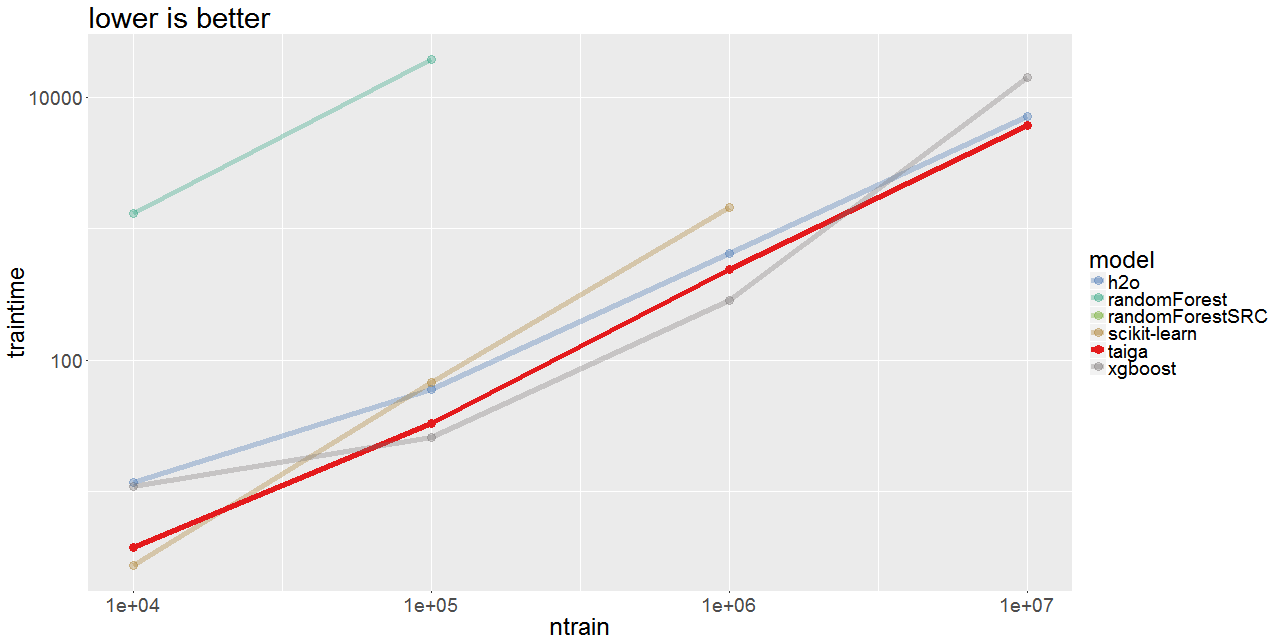
\includegraphics[width=16cm]{ontime/traintime.png}
\par\end{centering}
\protect\caption{\label{fig:ontime-traintime}Training time in seconds.}
\end{figure}

\begin{figure}[H]
\noindent \begin{centering}
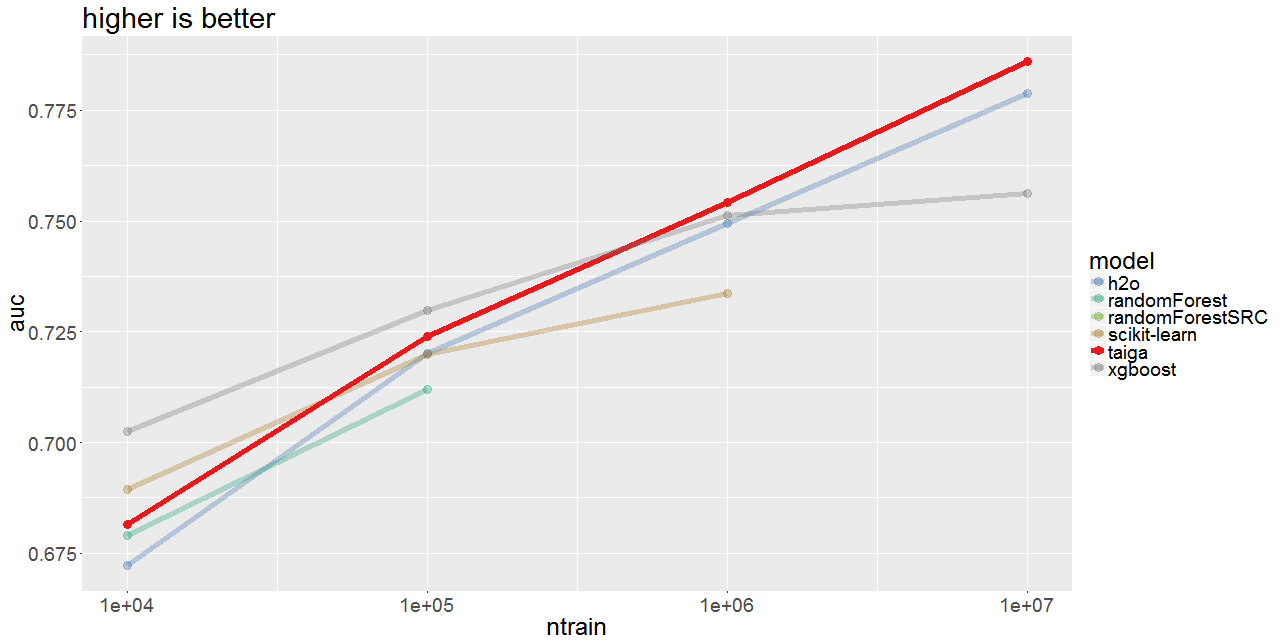
\includegraphics[width=16cm]{ontime/auc.png}
\par\end{centering}
\protect\caption{\label{fig:ontime-auc}Area under the ROC curve.}
\end{figure}


This section uses 
\href{http://stat-computing.org/dataexpo/2009/}
{public data on airline on-time performance} 
from the Data Expo poster session at the
$2009$ Joint Statistical Meetings.
The non-Taiga benchmarking code is inspired by Szilard Pafka's
\href{http://datascience.la/benchmarking-random-forest-implementations/}
{Benchmarking random forest implementations}.
(See also the
\href{https://www.r-bloggers.com/benchmarking-random-forest-implementations/}
{R-Bloggers version}
and the \href{https://github.com/szilard/benchm-ml}
{original benchmarking code}).

%\bibliographystyle{plainurl}
%\bibliography{bib,cactus}

\end{document}
